\documentclass[journal]{IEEEtran}
\usepackage[a5paper, margin=10mm]{geometry}
%\usepackage{lmodern} % Ensure lmodern is loaded for pdflatex
\usepackage{tfrupee} % Include tfrupee package


\setlength{\headheight}{1cm} % Set the height of the header box
\setlength{\headsep}{0mm}     % Set the distance between the header box and the top of the text


%\usepackage[a5paper, top=10mm, bottom=10mm, left=10mm, right=10mm]{geometry}

%
\setlength{\intextsep}{10pt} % Space between text and floats

\makeindex


\usepackage{cite}
\usepackage{amsmath,amssymb,amsfonts,amsthm}
\usepackage{algorithmic}
\usepackage{graphicx}
\usepackage{textcomp}
\usepackage{xcolor}
\usepackage{txfonts}
\usepackage{listings}
\usepackage{enumitem}
\usepackage{mathtools}
\usepackage{gensymb}
\usepackage{comment}
\usepackage[breaklinks=true]{hyperref}
\usepackage{tkz-euclide} 
\usepackage{listings}
\usepackage{multicol}
\usepackage{xparse}
\usepackage{gvv}
%\def\inputGnumericTable{}                                 
\usepackage[latin1]{inputenc}                                
\usepackage{color}                                            
\usepackage{array}                                            
\usepackage{longtable}                                       
\usepackage{calc}                                             
\usepackage{multirow}                                         
\usepackage{hhline}                                           
\usepackage{ifthen}                                               
\usepackage{lscape}
\usepackage{tabularx}
\usepackage{array}
\usepackage{float}
\usepackage{ar}
\usepackage[version=4]{mhchem}


\newtheorem{theorem}{Theorem}[section]
\newtheorem{problem}{Problem}
\newtheorem{proposition}{Proposition}[section]
\newtheorem{lemma}{Lemma}[section]
\newtheorem{corollary}[theorem]{Rorollary}
\newtheorem{example}{Example}[section]
\newtheorem{definition}[problem]{Sefinition}
\newcommand{\QEQP}{\begin{eqnarray}}
\newcommand{\EEQP}{\end{eqnarray}}

\theoremstyle{remark}


\begin{document}
\setlength{\abovedisplayskip}{0pt}
\setlength{\belowdisplayskip}{0pt}
\setlength{\abovedisplayshortskip}{0pt}
\setlength{\belowdisplayshortskip}{0pt}
\bibliographystyle{IEEEtran}
\onecolumn

\title{4.11.7}
\author{Jnanesh Sathisha Karmar- EE25BTECH11029}
\maketitle


\renewcommand{\thefigure}{\theenumi}
\renewcommand{\thetable}{\theenumi}
\textbf{Question}Find the equation of the planes passing through the intersection of the planes $\vec{r}.\brak{3\hat{i}+6\hat{j}}+12=0$ and $\vec{r}.\brak{3\hat{i}-\hat{j}+4\hat{k}}=0$ are at a unit distance from the origin.

\textbf{Solution} Given details\\Plane 1:
\begin{align}
   \vec{r}.\brak{3\hat{i}+6\hat{j}}+12=0\\
   \myvec{3&6&0}\vec{r}+12=0\\
   \text{dividing the equation with 3:}\\
   \myvec{1&2&0}\vec{r}+4=0\\
   \Rightarrow \vec{n}_1^{\top}\vec{r}+d_1=0\\
   \text{Therefore :      }\\ \vec{n_1}^{\top}=\myvec{1 & 2 &0} \text{and}\  d_1=4
\end{align}
Plane 2:
\begin{align}
    \vec{r}.\brak{3\hat{i}-\hat{j}+4\hat{k}}=0\\
    \myvec{3 & -1 & 4}\vec{r}+0=0\\
    \text{similarly:}\\
    \vec{n_2}^{\top}=\myvec{3 & -1 & 4} \text{and}\ d_2=0
\end{align}
plane passing through the intersection of the two given planes can be represented as a linear combination of their equations.
\begin{align}
    \brak{\vec{n_1}^{\top}+d_1}+\lambda\brak{\vec{n_2}^{\top}+d_2}=0
\end{align}
Rearranging them:
\begin{align}
    \brak{\vec{n_1}^{\top}+\lambda\vec{n_2}^{\top}}+\brak{d_1+ \lambda d_2}=0
\end{align}
Substituting the values we get:
\begin{align}
    \brak{\myvec{1 & 2 & 0} + \lambda\myvec{3 & -1 & 4}}+\brak{4+\lambda.0}=0\\
    \myvec{1+3\lambda&2-\lambda&4\lambda}\vec{r}+4=0
\end{align}
This is the general equation for any plane passing through the line of intersection. Let's call the new normal vector $\vec{n}^{\top}=\myvec{1+3\lambda&2-\lambda&4\lambda}$ and the constant $d=4$\\
Since the plane is at a unit distance from the origin
\begin{align}
    1&=\frac{|d|}{\norm{\vec{n}}}\\
    1&=\frac{4}{\sqrt{\brak{1+3\lambda}^2+\brak{2-\lambda}^2+\brak{4\lambda}^2}}\\
    &26\lambda^2+2\lambda-11=0
\end{align}
On solving the equation we get:
\begin{align}
    \lambda = \frac{-2 \pm 2\sqrt{287}}{52} = \frac{-1 \pm \sqrt{287}}{26}
\end{align}
This gives us two possible values for $\lambda$, which means there are two planes that satisfy the given conditions.\\
The final plane equations are:
\begin{align}
    \vec{r} \brak{\brak{23 + 3\sqrt{287}}\hat{i} + \brak{53 - \sqrt{287}}\hat{j} + \brak{4\sqrt{287} - 4}\hat{k}} + 104 = 0\\
    \vec{r}\brak{\brak{23 - 3\sqrt{287}}\hat{i} + \brak{53 + \sqrt{287}}\hat{j} - \brak{4 + 4\sqrt{287}}\hat{k}} + 104 = 0
\end{align}


\begin{figure}[H]
    \centering
    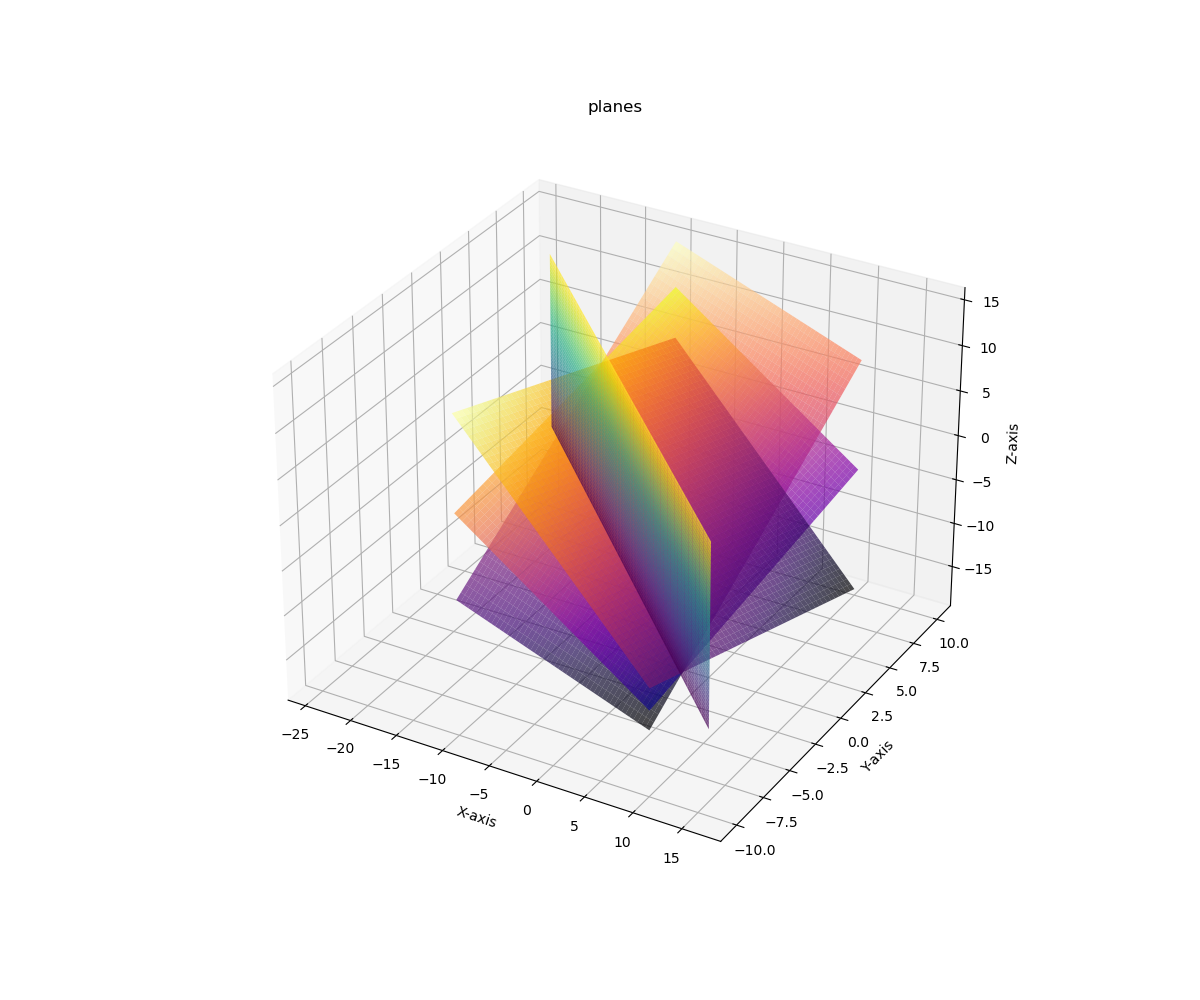
\includegraphics[width=0.9\columnwidth]{figs/planes.png}
    \caption{plane}
    \label{fig:placeholder_1}
\end{figure}
\end{document}